\begin{figure}
\centering
%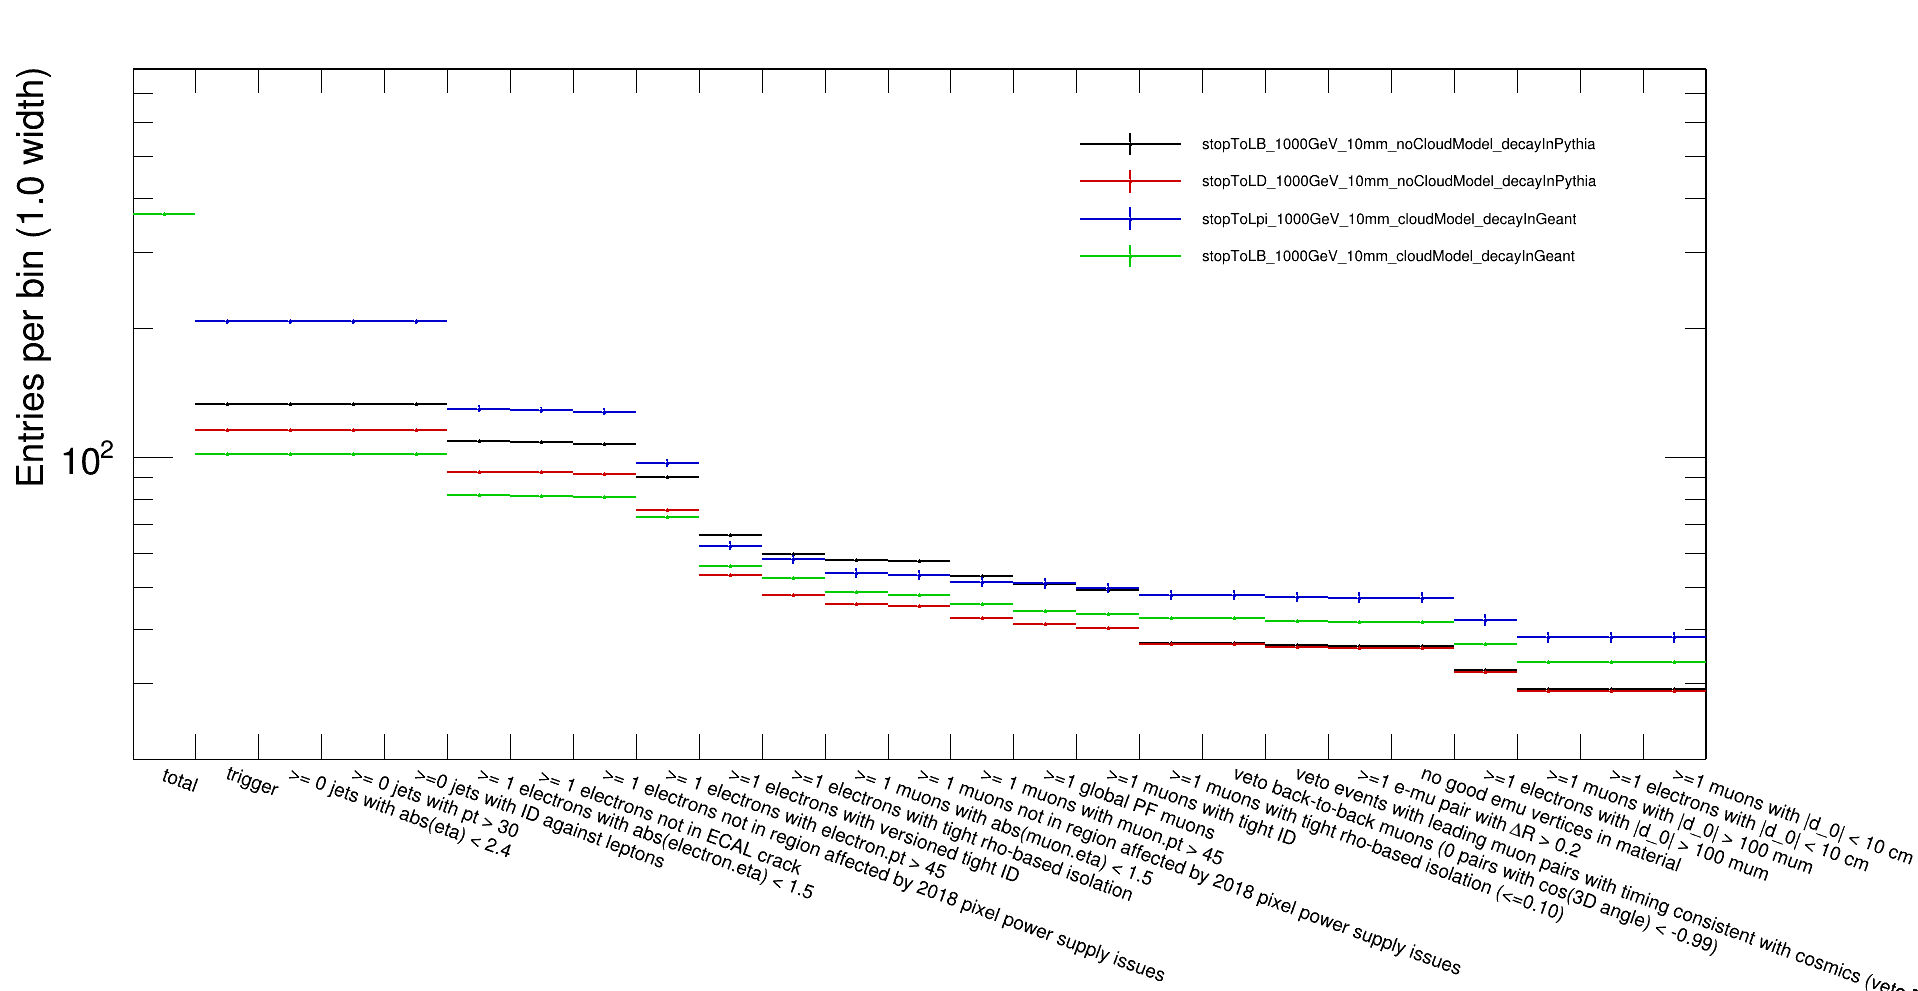
\includegraphics[width=0.78\textwidth]{figures/r_hadrons/emu_cutFlows_lb_ld_lpi_l_1000GeV_10mm.pdf}
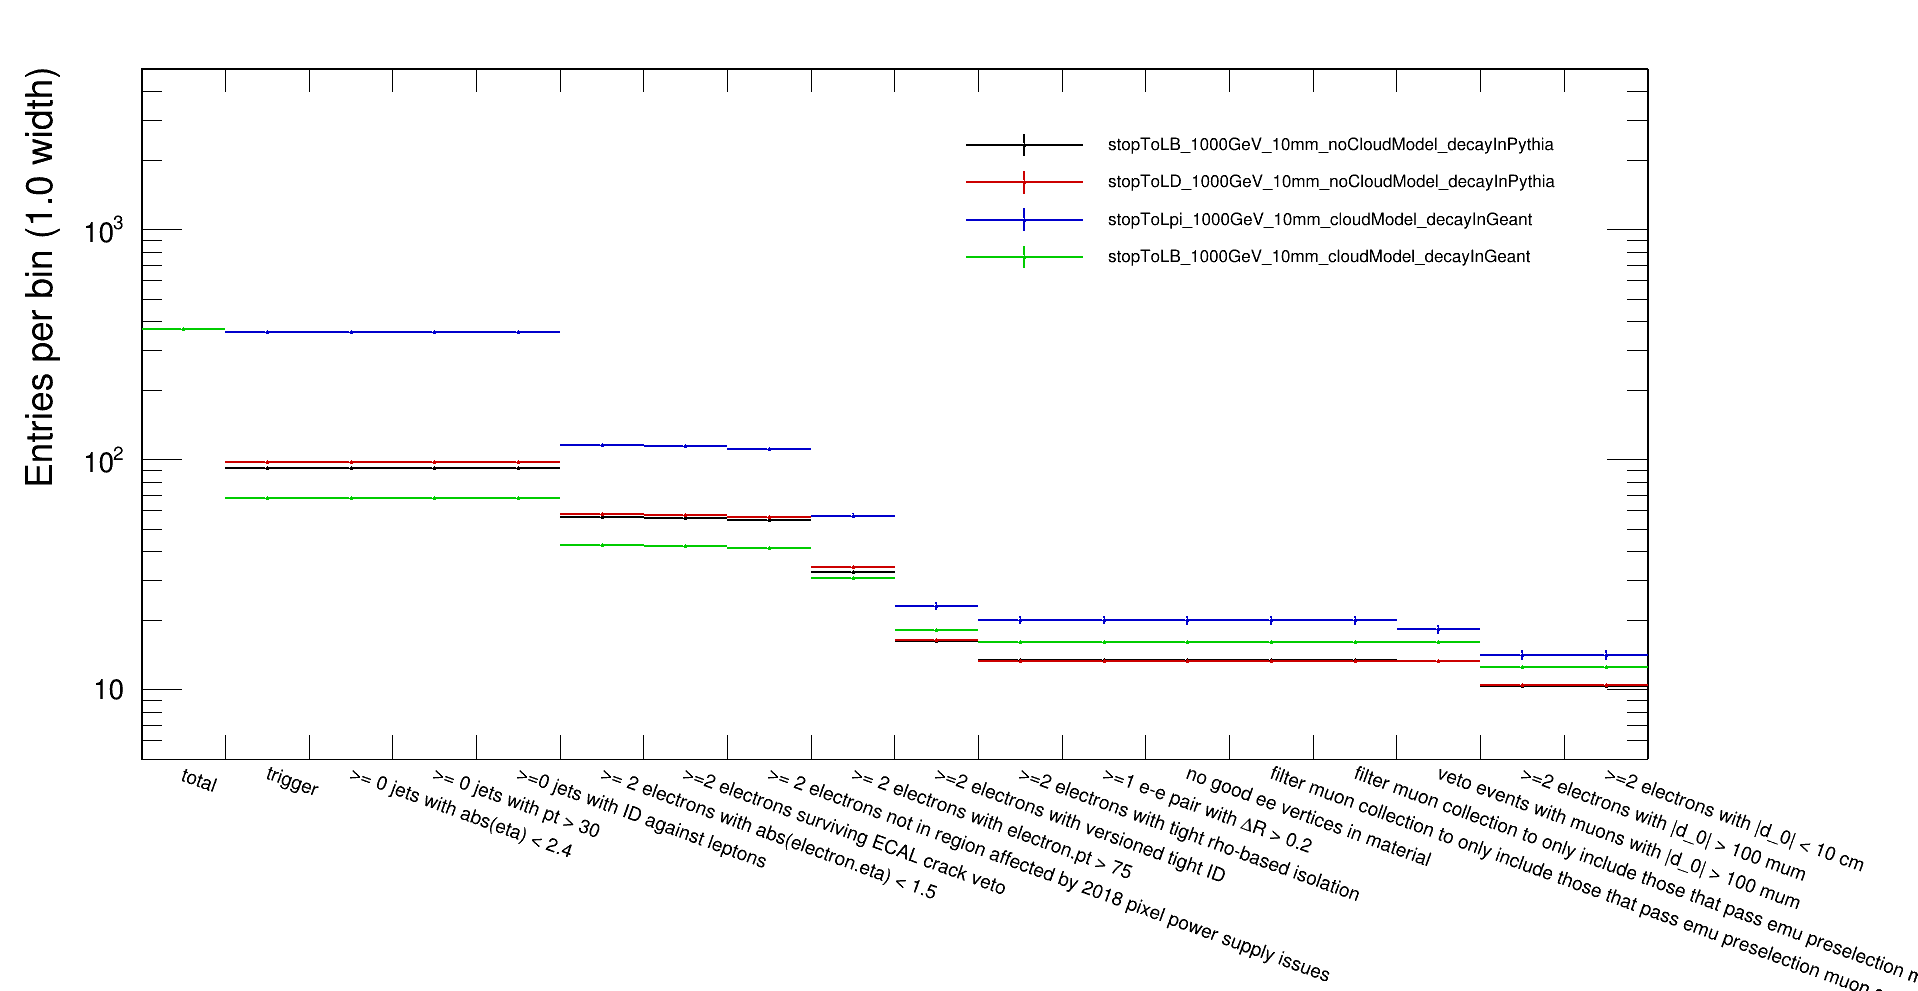
\includegraphics[width=0.9\textwidth]{figures/r_hadrons/ee_cutFlows_lb_ld_lpi_l_1000GeV_10mm.pdf}
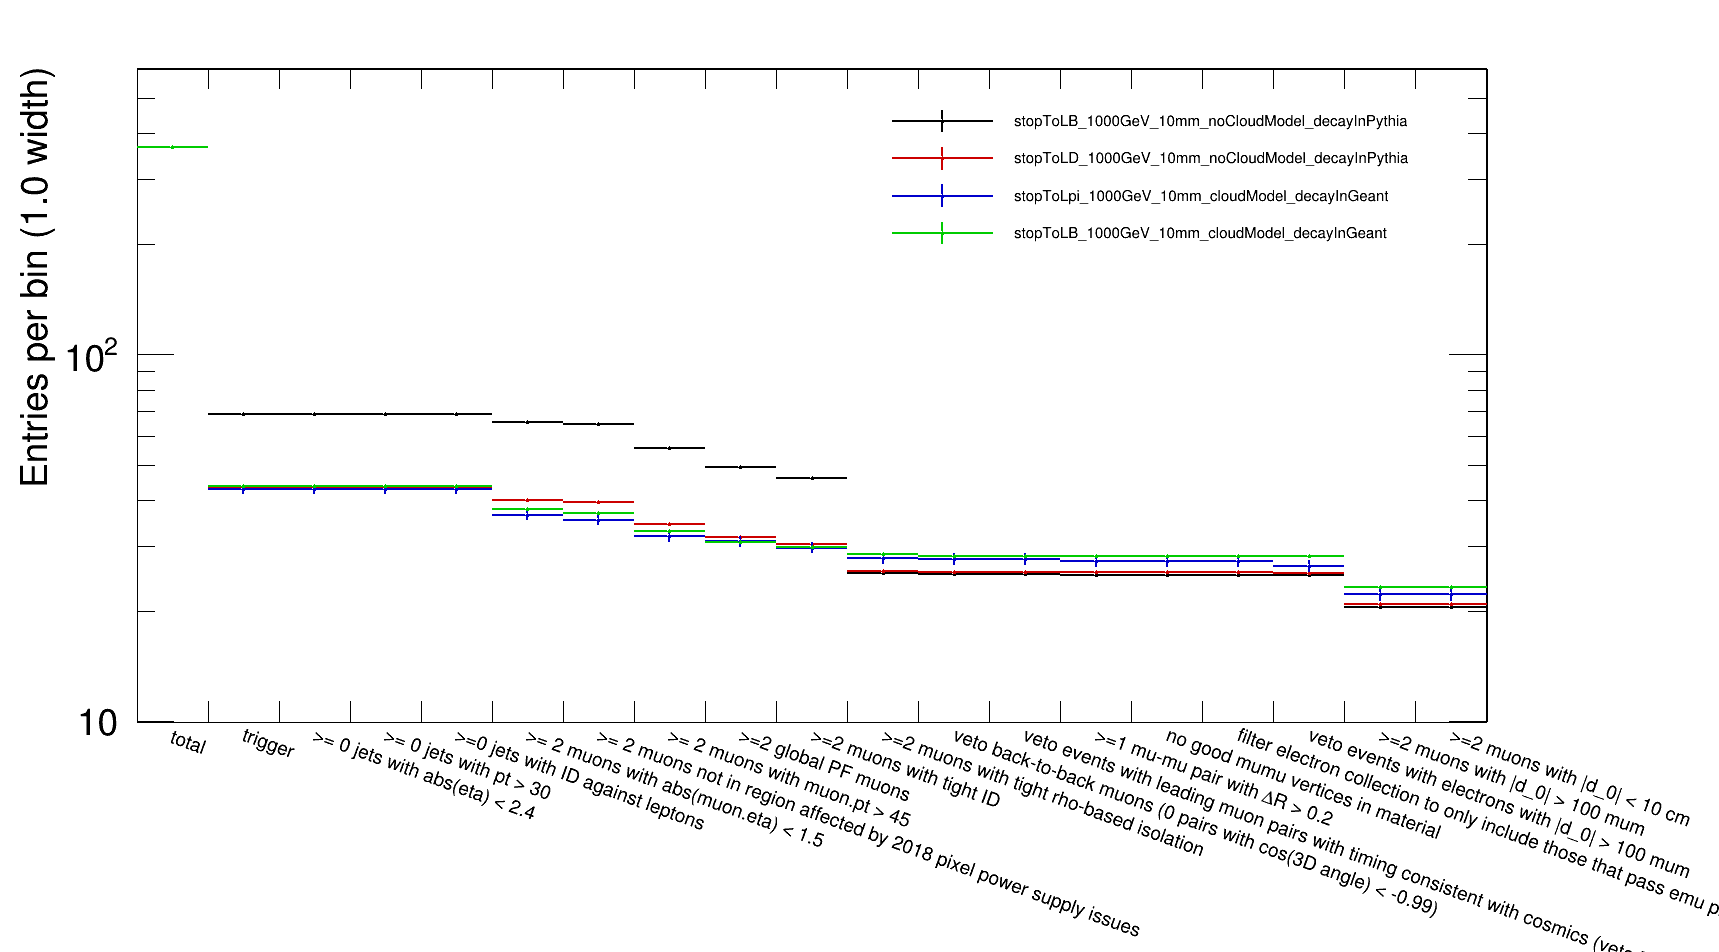
\includegraphics[width=0.9\textwidth]{figures/r_hadrons/mumu_cutFlows_lb_ld_lpi_l_1000GeV_10mm.pdf}
\caption{
Inclusive signal region cutflows for four signal samples  in the $\Pe\Pe$ (top) and $\Pgm\Pgm$ (bottom) channels. The top squark mass and proper decay length are 1000\GeV and 1\cm. In the sample corresponding to the black (red) curves, R-hadron material interactions are not modeled, but the top squark decay is performed in \PYTHIA and the resulting b (d) quark produces a jet. In the samples corresponding to the blue and green curves, the R-hadron material interactions and decay are modeled with \GEANTfour. In the sample corresponding to the blue curves, the R-hadron decays to a lepton and a neutral pion, and in the sample corresponding to the green curves, the R-hadron decays to a lepton and a non-physical final-state quark.
}
\label{r_hadron_cutflows}
\end{figure}